% !TEX TS-program = pdflatex
% !TEX encoding = UTF-8 Unicode

% This is a simple template for a LaTeX document using the "article" class.
% See "book", "report", "letter" for other types of document.

\documentclass[11pt]{article} % use larger type; default would be 10pt

\usepackage[utf8]{inputenc} % set input encoding (not needed with XeLaTeX)

%%% Examples of Article customizations
% These packages are optional, depending whether you want the features they provide.
% See the LaTeX Companion or other references for full information.

%%% PAGE DIMENSIONS
\usepackage{geometry} % to change the page dimensions
\geometry{a4paper} % or letterpaper (US) or a5paper or....
% \geometry{margin=2in} % for example, change the margins to 2 inches all round
% \geometry{landscape} % set up the page for landscape
%   read geometry.pdf for detailed page layout information

\usepackage{graphicx} % support the \includegraphics command and options

% \usepackage[parfill]{parskip} % Activate to begin paragraphs with an empty line rather than an indent

%%% PACKAGES
\usepackage{booktabs} % for much better looking tables
\usepackage{array} % for better arrays (eg matrices) in maths
\usepackage{paralist} % very flexible & customisable lists (eg. enumerate/itemize, etc.)
\usepackage{verbatim} % adds environment for commenting out blocks of text & for better verbatim
\usepackage{subfig} % make it possible to include more than one captioned figure/table in a single float
% These packages are all incorporated in the memoir class to one degree or another...

%%% HEADERS & FOOTERS
\usepackage{fancyhdr} % This should be set AFTER setting up the page geometry
\pagestyle{fancy} % options: empty , plain , fancy
\renewcommand{\headrulewidth}{0pt} % customise the layout...
\lhead{}\chead{}\rhead{}
\lfoot{}\cfoot{\thepage}\rfoot{}

%%% SECTION TITLE APPEARANCE
\usepackage{sectsty}
\allsectionsfont{\sffamily\mdseries\upshape} % (See the fntguide.pdf for font help)
% (This matches ConTeXt defaults)

%%% ToC (table of contents) APPEARANCE
\usepackage[nottoc,notlof,notlot]{tocbibind} % Put the bibliography in the ToC
\usepackage[titles,subfigure]{tocloft} % Alter the style of the Table of Contents
\renewcommand{\cftsecfont}{\rmfamily\mdseries\upshape}
\renewcommand{\cftsecpagefont}{\rmfamily\mdseries\upshape} % No bold!

%%% END Article customizations

%%% The "real" document content comes below...

\title{Juego BuscaMajinBoo}
\author{Lozano E. , Alvarado J \& .Lasso H.}
%\date{} % Activate to display a given date or no date (if empty),
         % otherwise the current date is printed 

\begin{document}
\maketitle

\section{Introducción}
El proyecto trata sobre la implementación  de un juego llamado BuscaMajinBoo, cuyo propósito es poder usar el lenguaje Java  para  realizar aplicaciones de forma ``nativa” en la plataforma de Android. Haciendo uso de nuestra experiencia en este lenguaje.\\
Android es un sistema operativo utilizado por  teléfonos inteligentes con pantalla táctil y en tablets. Actualmente hay más de 100.000  aplicaciones gratuitas disponibles para android, por este motivo es uno de los sistemas operativos para teléfonos inteligentes  más usados en el mundo.\\ \\
BuscaMajinBoo se basa en la reglas de juego del buscaminas tradicional pero tiene el fin de presentar un tema de un anime conocido como lo es`` DGBZ" haciéndolo a su vez mas interesante, y aun más si está implementado para dispositivos Android.

\section{Alcance}
El alcance de nuestro proyecto es realizar una aplicación dirigida a los dispositivos android, específicamente Tablets. \\
La aplicación consistirá en el juego conocido como "Buscaminas" y todas sus funcionalidades.\\
La programación del juego requerirá entender el Modelo Vista Controlador que maneja el SDK de android y familiarizarnos con la sintáxis de XML. 

\section{Descripción}
El juego consiste es descubrir todas las celdas del tablero que no se encuentre el Majin  Boo.
El juego consta de  diferentes dificultades, cada dificultad posee un tablero con un tamaño específico y un número de minas designado, las dificultades son las siguientes:\\
\begin{itemize}
\item Beginner:Muestra un tablero de dimensión 5x5, con 5 minas.\\
\item Intermediate:Muestra un tablero de dimensión 8x8 con 10 minas\\
\item Advanced:Muestra un tablero de dimensión 11x11 con 20 minas \\
\item  Custom:El jugador escoge las dimensiones del tablero con la cantidad de minas respectivas\\
\end{itemize}
\subsection{Reglas del Juego}
\begin{itemize}
\item Cuando la celda descubierta contiene un Majin Boo el jugador pierde  presentando el mensaje ``BOOM".
\item Si la celda descubierta contiene un número el usuario puede seguir jugando.
\item Si la celda descubierta se encuentra vacía, es decir no contiene ni un número ni una mina, se descubren todas las celdas
adyacentes a ella que están vacías o contienen números.
\item Un celda tiene adyacencia con las 8 celdas a su alrededor.
\item El juego finalizará cuando todos los casilleros que no contienen minas han sido descubiertos y se le presentara un mensaje al jugador diciendo “Ganaste” y si el tiempo de juego se encuentra entre los 3 primeros se le pedirá el nombre del jugador para registrarlo entre los mejores tiempos.
\end {itemize}

\section{Manual}
Al iniciar el juego nos encontramos con el menu principal. Donde podremos escoger 3 opciones:
\begin{center}
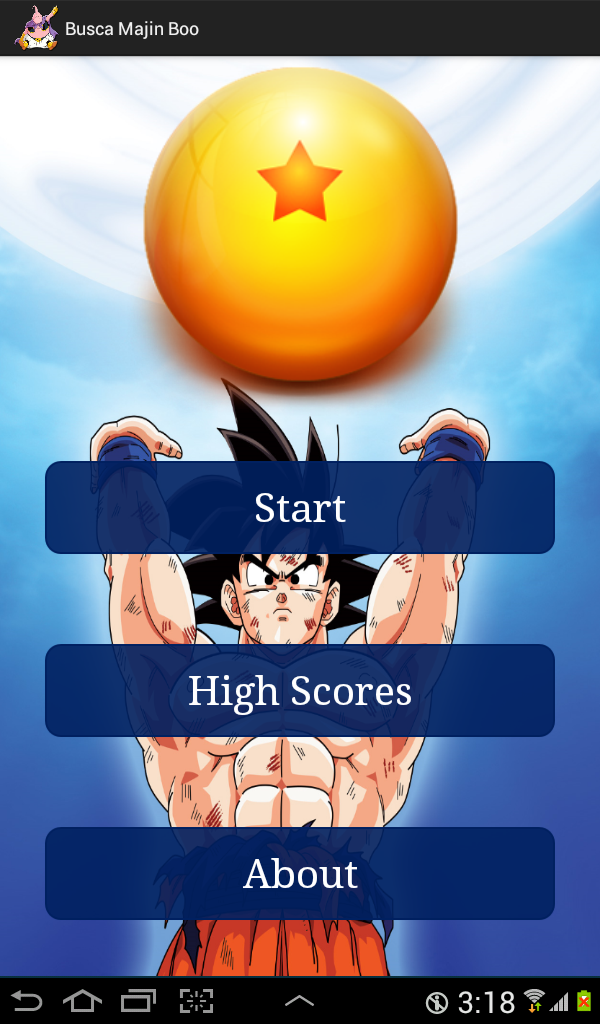
\includegraphics[scale=0.15]{Imagenes/SSMenuPrincipal.png}
\end{center}
\subsection{Iniciar Partida}
En este menu podemos escoger entre 3 dificultades prediseñadas y una dificultad personalizable
\begin{center}
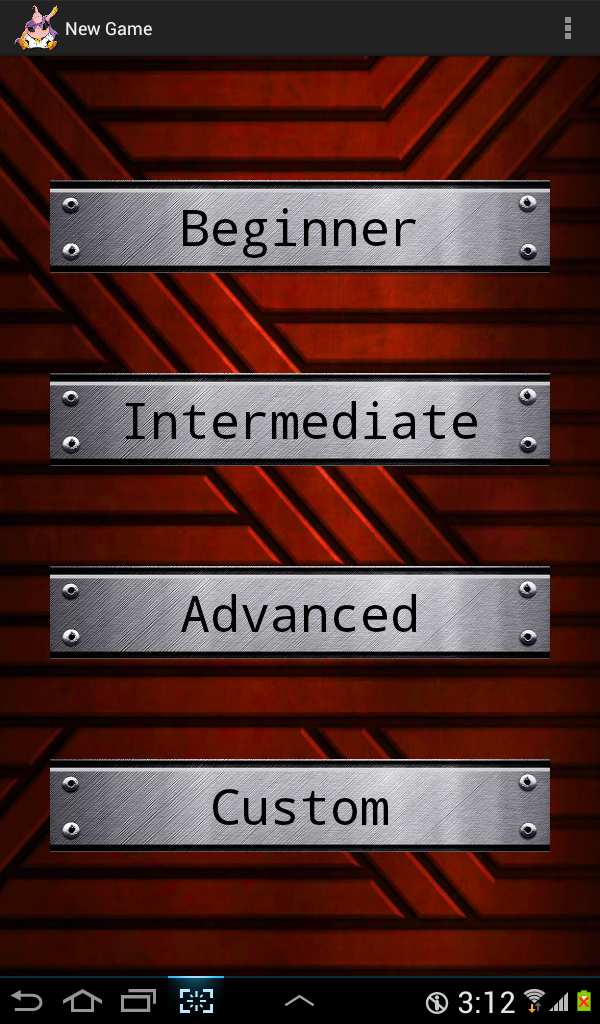
\includegraphics[scale=0.2]{Imagenes/SSMenuNewGame.png}
\end{center}
\begin{itemize}
\item Beginner:Muestra un tablero de dimensión 5x5, con 5 minas.\\
\begin{center}
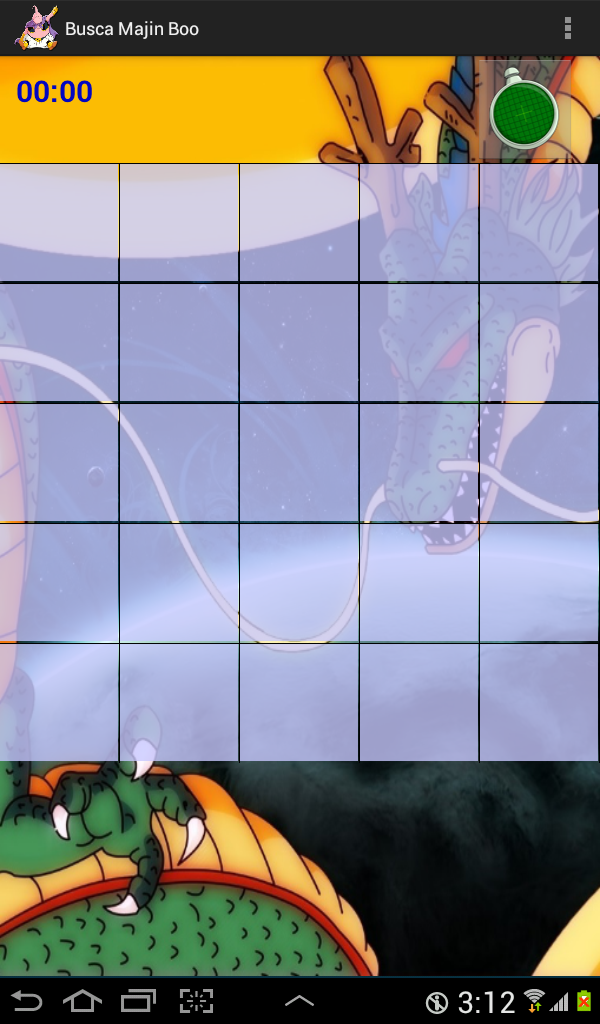
\includegraphics[scale=0.2]{Imagenes/SSEasy.png}
\end{center}
\item Intermediate:Muestra un tablero de dimensión 8x8 con 10 minas\\
\begin{center}
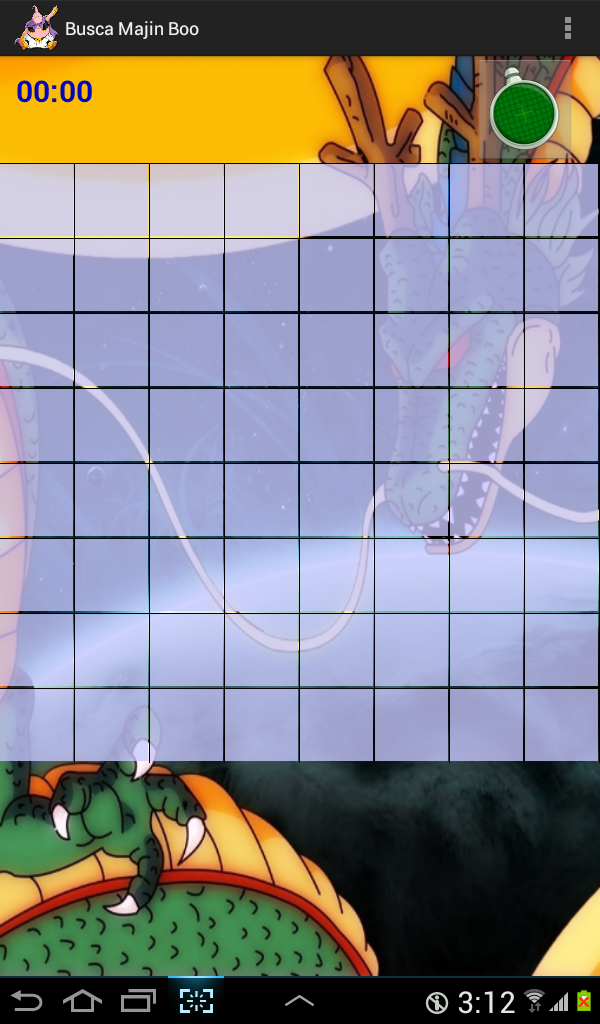
\includegraphics[scale=0.2]{Imagenes/SSNormal.png}
\end{center}
\item Advanced:Muestra un tablero de dimensión 11x11 con 20 minas \\
\begin{center}
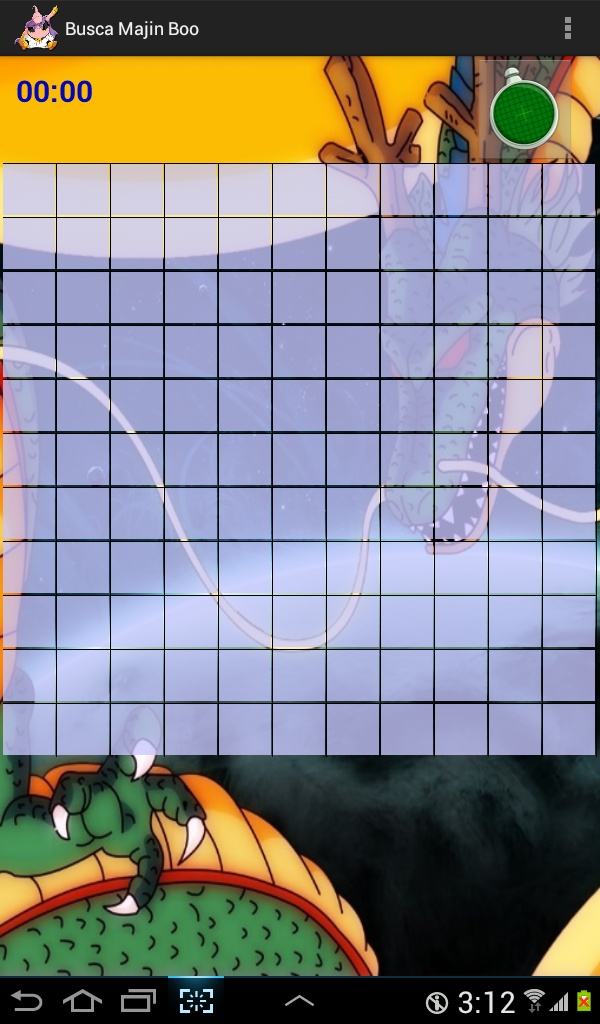
\includegraphics[scale=0.2]{Imagenes/SSHard.png}
\end{center}
\end {itemize}
\subsubsection{Partida personalizada}
Esta opcion nos permite escoger numero de celdas del tablero (ancho y alto) y el numero de minas.
\begin{center}
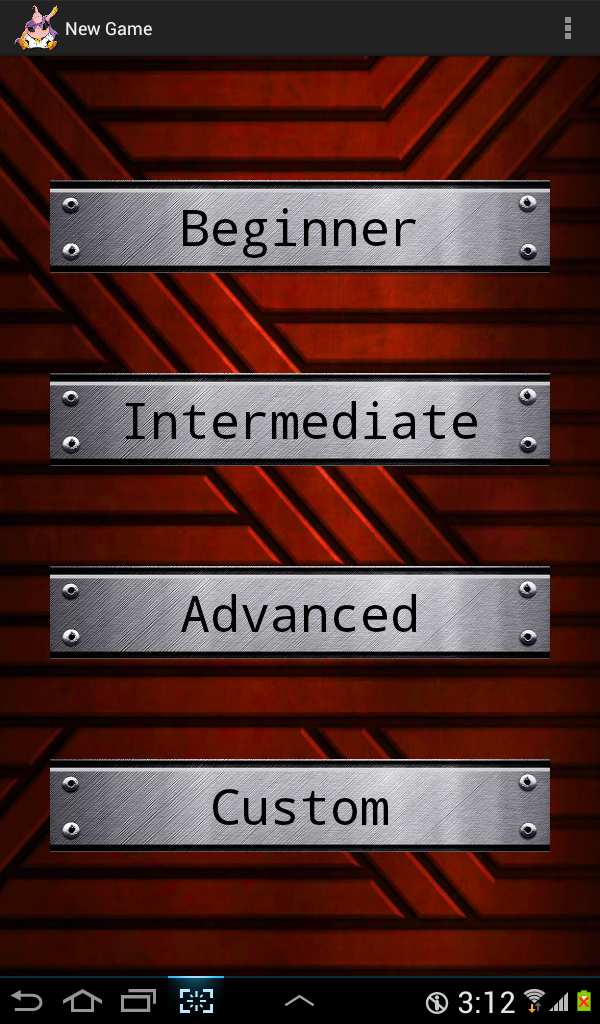
\includegraphics[scale=0.2]{Imagenes/SSMenuNewGame.png}
\end{center}
\subsection{Revisasr Puntuaciones Maximas}
Este menu nos permite revisar los mejores tiempos guardados, ademas de darnos la opcion de resetear los tiempos.
\begin{center}
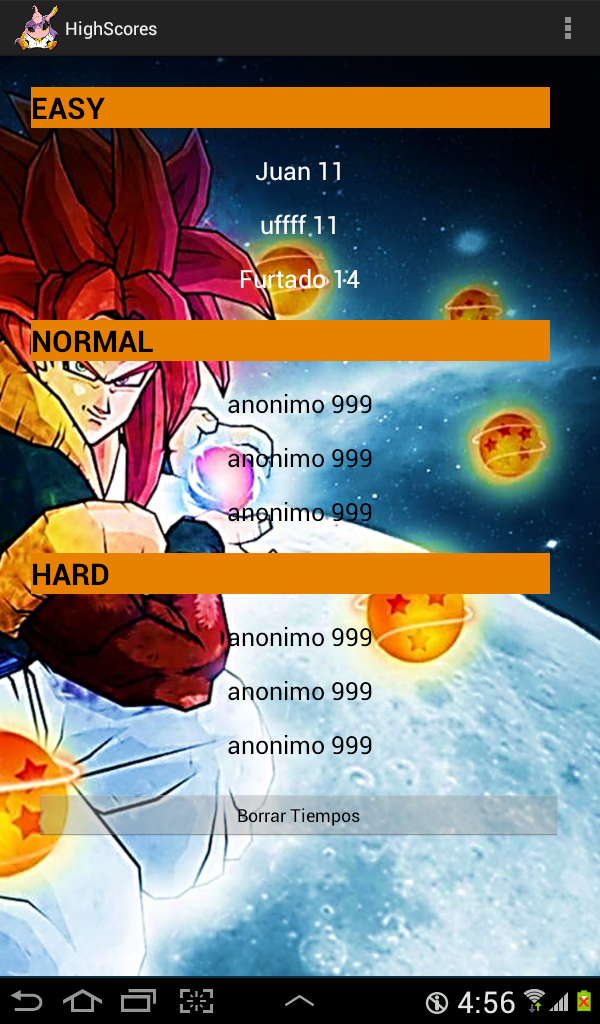
\includegraphics[scale=0.2]{Imagenes/SSHighScores.png}
\end{center}
\subsection{Acerca de}
Este menu nos muestra informacion acerca de la aplicación
\begin{center}
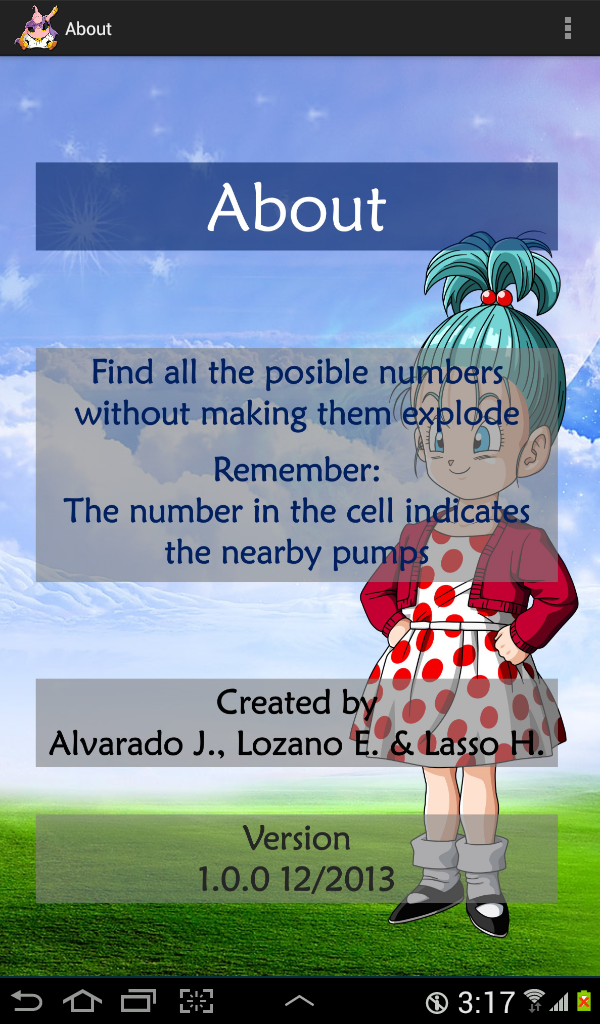
\includegraphics[scale=0.2]{Imagenes/SSAbout.png}
\end{center}

\section{¿Qué se implementó y qué no se implementó? }
\subsection{Lo implementado} 
\begin{itemize}
\item El juego permite escoger diferentes tamaños del tablero de acuerdo a tres dificultades y a un nivel ``Custom"; en el cuál el jugador podrá establecer el ancho, alto y número de minas deseado.
\item El jugador puede visualizar desde el menú principal los Altos Puntajes en los diferentes niveles del juego, y de la misma forma podrá dejar limpio el registro de puntuaciones.
\item Una vez el tablero se encuentre dibujado en la nueva partida, el jugador tiene dos diferentes acciones de juego, un ``Clik" corto y uno largo. Con el corto el juego permite descubrir la celda y con el largo permite colocar un Mr. Satán sobre la celda.
\item El juego permite que al dar el primer ``Clik" el jugador no se encuentre con un Majin Boo.
\item También se ha implementado un Cronómetro, que comienza cuando el jugador da el primer ``Clik"; ya sea éste largo o corto.
\item El cronómetro es el que establece si un jugador al ganar una partida merece o no guardar su puntuación. Ya que al finalizar la partida Ganada se verifica si el tiempo transcurrido es menor a los que se encuentrar registrados en las puntuaciones. Y si es así se solicita el juego permite solicitar el nombre del jugador y de ésta forma registrarlo.
\item El tablero posee un Radar que le permitirá al jugador reiniciar el tablero cuando desee.
\item El tablero al dar el primer ``Clik" se colocan los Majin Boos. Y una vez comenzada la partida, el juego usa recursión para determinar el contenido de cada celda. El contenido varía de 0 a 8 y 80. donde 0 es que la celda no tiene Majin Boos adyacentes, 80 que la celda está ocupada por un Majin Boo y el contenido en el rando de 1 a 8 depende de los adyacentes.
\item Una vez el jugador haya perdido la partida se muestran todos los Majin Boo escondidos y finaliza el juego.
\item Una vez el jugador haya ganado la partida se muestran todos los Mr. Satán donde estaban los Majin Boo escondidos y finaliza el juego.
\end {itemize}

\subsection{Lo NO implementado} 
\begin{itemize}
\item El juego no permite rotación de la pantalla debido a falta de tiempo de programación. 
\end {itemize}

\section{Observaciones}
\begin{itemize}
\item Aprender sobre el funcionamiento del SDK de Android fue lo que más demoró el comienzo de la programación del proyecto.
\item Hay que mejorar el uso de Git ya que se presentaron varios problemas para subir los cambios al repositorio que afectaban la misma linea del código.
\end{itemize}
\section{ Conclusiones}

\begin{itemize}
\item Debido al avance tecnólogico y de la aceptación de los dispositivo android es necesario tener conocimiento de la implementación de las aplicaciones para este sistema operativo.
\item La popularidad de android ofrece una gran documentación en Internet sobre uso, ejemplos, librerias, etc. Que facilitan la tarea del programador si es un buen investigador.
\item Es fundamental para un programador entender cómo el SDK de android usa el Modelo Vista Controlador para poder relacionar los XML de los layouts y las clases en Java.
\item El trabajo en equipo se mejoró con el uso de la herramienta GitHub. Gracias a sus funcionalidades y a sus herramientas.
\item Algunos de nosotros no somos observadores, ya que tuvimos que jugar buscaminas unas cuantas veces para poder entender bien el juego, que Windows nos ha permitido jugar muchas veces.

\end {itemize}



\end{document}
